\id{МРНТИ 54.37.15}{https://doi.org/10.58805/kazutb.v.2.27-954}
\vspace{-0.5em}
\begin{articleheader}
\sectionwithauthors{О.В. Рожкова, О.О. Ковалева, В.И. Лебедева, Д.А. Ветюгов, В.И. Рожков}{ИССЛЕДОВАНИЕ ПРОЦЕССА ОКОМКОВАНИЯ ВЫСОКОКАЧЕСТВЕННОГО ЖЕЛЕЗОРУДНОГО КОНЦЕНТРАТА С ПРИМЕНЕНИЕМ НОВЫХ СВЯЗУЮЩИХ ДОБАВОК}

{\bfseries
\textsuperscript{1,2,3}О.В. Рожкова\alink{https://orcid.org/0000-0001-8163-7035}\textsuperscript{\envelope },
\textsuperscript{1}О.О. Ковалева\alink{https://orcid.org/0009-0002-5015-5265},
\textsuperscript{4}В.И. Лебедева\alink{https://orcid.org/0009-0001-3003-5760},
\textsuperscript{5}Д.А. Ветюгов\alink{https://orcid.org/0009-0009-9880-6259},
\textsuperscript{2}В.И. Рожков\alink{https://orcid.org/0000-0002-3232-5972}
}
\end{articleheader}

\begin{affiliation}
\textsuperscript{1}ТОО «Алтайский геолого-экологический институт», г. Усть-Каменогорск, Казахстан,

\textsuperscript{2}НАО «Казахский~агротехнический исследовательский университет им.~С.~Сейфуллина», г. Астана, Казахстан,

\textsuperscript{3}АО «Science and Technology Solutions», г. Алматы, Казахстан,

\textsuperscript{4}ООО «Бентонит Хакасии», г. Черногорск, Россия,

\textsuperscript{5}ООО «Компания Бентонит», г. Москва, Россия

\raggedright \textsuperscript{\envelope }Корреспондент-автор: rozhkova.o@stsolutions.kz
\end{affiliation}

Одной из важнейших задач в подготовке сырья при производстве окатышей
для металлургического передела является управление качеством, которое
можно осуществлять путем изменения состава шихты, введения ряда
связующих добавок, а также процессом термообработки.

В данной статье приведены результаты применения высококачественных
связующих для получения железорудных окатышей с высокой прочностью на
сжатие и низким сопротивлением к истиранию.

Результаты, полученные в ходе тестовых лабораторных испытаний по выбору
типа связующих ТОО «Тагбент» для окомкования концентрата АО
«Соколовско-Сарбайское горно-обогатительное производственное
объединение» (АО «ССГПО», Казахстан), указывают, что физико-механические
свойства обожженных окатышей зависят от комплекса факторов, среди
которых важнейшим является качество сырых окатышей напрямую связанных со
свойствами связующих добавок.

Показано, что рекомендуемые связующие добавки производства ТОО «Тагбент»
(Казахстан, Тарбагатайский район с. Акжар) и бенто-полимерной композиции
(БПК) при расходе в шихте 0,49 - 0,50 \% позволяют стабилизировать
гранулометрический состав сырых окатышей, улучшить прочностные
характеристики сырых, и улучшить показатель сопротивления истиранию
обожженных окатышей.

Анализ качественных характеристик готовой продукции, выявил линейную
зависимость с удельным расходом бентонита, оптимизация которого
позволяет обеспечивать заданные показатели качества железорудных
окатышей.

{\bfseries Ключевые слова:} бенто-полимерная композиция, концентрат,
технология, процесс окомкования, железорудная шихта.

\begin{articleheader}
{\bfseries ЖАҢА БАЙЛАНЫСТЫРУШЫ ҚОСПАЛАРДЫ ҚОЛДАНУ АРҚЫЛЫ ЖОҒАРЫ САПАЛЫ ТЕМІР КЕНІ КОНЦЕНТРАТЫН ТҮЙІРШІКТЕУ ПРОЦЕСІН ЗЕРТТЕУЫ}

{\bfseries
\textsuperscript{1,2,3}О.В. Рожкова\textsuperscript{\envelope },
\textsuperscript{1}О.О. Ковалева,
\textsuperscript{4}В.И. Лебедева,
\textsuperscript{5}Д.А. Ветюгов,
\textsuperscript{2}В.И. Рожков
}
\end{articleheader}

\begin{affiliation}
\textsuperscript{1}«Алтай геологиялық-экологиялық институты» ЖШС, Өскемен, Қазақстан,

\textsuperscript{2}«С.Сейфуллин атындағы Қазақ агротехникалық зерттеу университеті» ҰАО, Астана, Қазақстан,

\textsuperscript{3}«Science and Technology Solutions» АҚ, Алматы, Қазақстан,

\textsuperscript{4}«Бентонит Хакасия» ЖШС, Черногорск қ., Ресей,

\textsuperscript{5}«Компания Бентонит» ЖШС, Мәскеу, Ресей,

e-mail: rozhkova.o@stsolutions.kz
\end{affiliation}

Металлургиялық өңдеуге арналған түйіршіктер өндірісінде шикізатты
дайындаудағы маңызды міндеттердің бірі, шихтаның құрамын өзгерту,
бірқатар байланыстырушы қоспаларды енгізу, сондай-ақ термиялық өңдеу
процесі арқылы жүзеге асырылатын сапаны басқару.

Бұл мақалада қысу беріктігі жоғары және тозуға төзімділігі төмен темір
кені түйіршіктерін алу үшін жоғары сапалы байланыстырғыштарды қолдану
нәтижелері келтірілген.

"Соколов-Сарыбай тау-кен байыту өндірістік бірлестігі" АҚ ("ССКӨБ" АҚ,
Қазақстан) концентратын түйіршік түйістіру үшін "Тагбент" ЖШС
байланыстырушы түрін таңдау бойынша тестілік зертханалық сынақтар
барысында алынған нәтижелер күйдірілген түйіршіктердің
физикалық-механикалық қасиеттері факторлар кешеніне байланысты екенін
көрсетеді, олардың ішінде шикі түйіршіктердің сапасы байланыстырушы
қоспалардың қасиеттерімен тікелей байланысы аса маңызды болып табылады.

"Тағбент" ЖШС (Қазақстан, Ақжар ауылы Тарбағатай ауданы) және
Бенто-полимерлі композиция (БПК) өндірісінің 0,49 - 0,50\% шихтада
тұтыну кезінде ұсынылатын байланыстырушы қоспалары шикі түйіршіктердің
гранулометриялық құрамын тұрақтандыруға, шикі түйіршіктердің беріктік
сипаттамаларын жақсартуға және күйдірілген түйіршіктердің тозуына
төзімділік көрсеткішін жақсартуға мүмкіндік беретіні көрсетілген.

Дайын өнімнің сапалық сипаттамаларын талдау бентониттің меншікті
шығынына сызықтық тәуелділікті анықтады, оны оңтайландыру темір кені
түйіршіктерінің сапасының берілген көрсеткіштерін қамтамасыз етуге
мүмкіндік береді.

{\bfseries Түйін сөздер:} бентополимер құрамы, концентрат, технология,
түйіршіктеу процесі, темір рудасының шихтасы.

\begin{articleheader}
{\bfseries RESEARCH OF THE PELLETIZATION PROCESS HIGH QUALITY IRON ORE CONCENTRATE USING NEW BINDING ADDITIVES}

{\bfseries
\textsuperscript{1,2,3} O.V. Rozhkova\textsuperscript{\envelope },
\textsuperscript{1}O.O. Kovaleva,
\textsuperscript{4}V.I. Lebedeva,
\textsuperscript{5}D.A. Vetyugov,
\textsuperscript{2}V.I. Rozhkov
}
\end{articleheader}

\begin{affiliation}
\textsuperscript{1}Altai Geological-Ecological Institute LLP, Ust-Kamenogorsk, Kazakhstan,

\textsuperscript{2}NAO ``Kazakh Agrotechnical Research University named after. S. Seifullin'', Astana, Kazakhstan,

\textsuperscript{3}JSC ``Science and Technology Solutions'', Almaty, Kazakhstan,

\textsuperscript{4} Bentonite Khakassia LLC, Chernogorsk, Russia,

\textsuperscript{5}LLC ``Company Bentonit'', Moscow, Russia,

e-mail: rozhkova.o@stsolutions.kz
\end{affiliation}

One of the most important tasks in the preparation of raw materials for
the production of pellets for metallurgical processing is quality
management, which can be carried out by changing the composition of the
charge, introducing a number of binding additives, as well as the heat
treatment process.

This article presents the results of using high-quality binders to
produce iron ore pellets with high compressive strength and low abrasion
resistance.

The results obtained during laboratory tests to select the type of
binders of «Tagbent» LLP for pelletizing concentrate of Sokolov-Sarbay
Mining Production Association JSC (SSGPO JSC, Kazakhstan) indicate that
the physical and mechanical properties of the fired pellets depend on a
set of factors, among which the most important is the quality of raw
pellets directly related to the properties of binding additives.

It has been shown that the recommended binding additives produced by
«Tagbent» LLP (Kazakhstan, Tarbagatai district, Akzhar village) and
bento-polymer composition (BPC) at a consumption in the charge of 0.49 -
0.50\% make it possible to stabilize the granulometric composition of
raw pellets, improve the strength characteristics of raw pellets, and
improve the abrasion resistance of fired pellets.

Analysis of the quality characteristics of the finished product revealed
a linear relationship with the specific consumption of bentonite, the
optimization of which allows us to ensure the specified quality
indicators of iron ore pellets.

{\bfseries Keywords:} bento-polymer composition, concentrate, technology,
pelletizing process, iron ore charge.
\vspace{-0.5em}
\begin{multicols}{2}
{\bfseries Введение.} Расширение рынка сбыта железорудного сырья вызывает
необходимость повышения конкурентоспособности продукции, подразумевая
улучшение потребительских свойств железорудных окатышей {[}1{]}.
Поскольку повышение
\href{https://www.yandex.ru/search/?text=\%D0\%BF\%D1\%80\%D0\%BE\%D1\%87\%D0\%BD\%D0\%BE\%D1\%81\%D1\%82\%D0\%BD\%D1\%8B\%D1\%85\%20\%D1\%81\%D0\%B2\%D0\%BE\%D0\%B9\%D1\%81\%D1\%82\%D0\%B2\%20\%20&lr=213&msid=1739867152.50217765.01245.11111&search_source=chromentp_desktop&suggest_reqid=163703149161131391771529680334996&msp=1}{прочностных свойств},
способность окатышей сопротивляться разрушению, достигается в том числе
качеством компонентов шихты, при подготовке сырья к металлургическому
переделу {[}2{]}. Такое управление можно осуществлять с помощью ряда
технологических приемов, выполняемых при подготовке шихты и в процессе
термообработки, а также путем изменения состава шихты за счет введения
ряда добавок.

Сырые окатыши формируются при окатывании тонкодисперсного железорудного
концентрата в специальных установках - окомкователях.

Процесс получения сырого окатыша помимо динамических нагрузок в
окомкователе определяется двумя основными типами сил - молекулярной и
капиллярной. Эти же типы сил определяют закономерности пропитки слоя
концентрата.

Масса тонкоизмельченного концентрата представляет собой сыпучее тело,
пронизанное капиллярами, образованное мелкими порами - промежутками
между частицами концентрата. В зависимости от размера пор и пористости
слоя концентрата одно и тоже количество воды, контактирующей с
концентратом, смачивает различные объёмы концентрата и по-разному
упрочняет увлажненные комки концентрата. Количество капиллярной влаги
может достигать 50\% и более в зависимости от пористости твердого
вещества и размера частиц. Размеры пор и общая пористость слоя
концентрата зависят как от гранулометрического состава концентрата, так
и связующего компонента.

Известно, что {[}3{]} характеризующим параметром процесса окомкования
является коэффициент комкуемости шихты. Эффективный радиус, и как
следствие, комкуемость концентрата, оказывает влияние на образование,
формирование и рост окатышей в процессе окомкования.

Процесс комкуемости {[}4{]} связанный со скоростью образования и роста
гранул характеризуется прочностью сцепления частиц в грануле, который
зависит от следующих факторов:

- содержания влаги в железорудной шихте (оптимальной влажностью является
такое содержание влаги в шихте, которое обеспечивает максимальный выход
годного класса);

- гранулометрического состава железорудного материала;

- удельной поверхности железорудного материала (которая тем больше, чем
выше содержание наиболее мелкой фракции). Увеличение удельной
поверхности концентрата ускоряет процесс окомкования;

- однородности шихты (заключается в правильном и точном дозировании
компонентов шихты). Правильность дозирования шихтовых материалов
обеспечивается расчетом шихты;

- условий образования гранул в окомкователе (степень заполнения, частота
вращения, состояние внутренней поверхности);

- вид связующего компонента.

Комкуемость является универсальным параметром, характеризующим
способность тонкодисперсных материалов к образованию прочных гранул
{[}5{]}. Чем выше показатель комкуемости шихты, тем равномернее
формируется размер сырых окатышей, т.е. выход годного класса в диапазоне
10÷14 мм в общей массе полученных сырых окатышей увеличивается.

Для увеличения прочности сырых и, особенно сухих окатышей, их ударной
прочности при быстром нагреве и интенсификации сушки на обжиговой
машине, для улучшения металлургических свойств окатышей применяют
связующие добавки {[}2{]}.

Роль связующих заключается не только в обеспечении прочности сырых
окатышей (достаточной для их транспортировки от окомкователя до
обжиговой машины), но и прочности сухих окатышей (что особенно важно для
интенсификации процесса сушки). При производстве окатышей из
глубокообогащенных концентратов связующие добавки активно участвуют в
формировании оптимальной структуры окатышей, определяющей в конечном
счете их качество и металлургические свойства.

Характерным свойством связующих является их высокая степень измельчения
и коллоидный характер {[}6{]}. Наиболее распространенным связующим при
производстве окатышей является бентонит. Основной составляющей
бентонитовых глин является монтмориллонит Аl\textsubscript{2}Озх
4SiO\textsubscript{2} хЗН\textsubscript{2}О. Это природный минерал и в
процессе переработки на его влиять невозможно.

Бентонит представляет собой высокодисперсную глину, способную набухать в
присутствии воды и коллоидного сцепления (клеящие свойства) частиц за
счет способности глины образовывать гель и образовывать большое
количество тонкодисперсных частиц, взаимодействующих с частицами
концентрата.

Частицы бентонита после увлажнения образуют пленку с большой
поверхностью, которая обволакивает частицы концентрата и соединяет их
между собой. Прочность сырых и, главное, высушенных окатышей с добавкой
бентонита повышается благодаря взаимному притяжению частиц бентонита и
притяжению частиц, бентонита и магнетита, причем связка сохраняется и
после удаления воды во время сушки. Прочность сухого окатыша
определяется энергией межфазных взаимодействий в системе: концентрат --
бентонит.

Применение бентонита улучшает комкуемость, повышает пластичность сырого
окатыша к динамическим нагрузкам, регулирует скорость дегидратации
окатышей, выделять при нагреве влагу в процессе сушки, что предохраняет
их от разрушения и получить обожженные окатыши необходимого качества.

В результате образования шлакового расплава возрастает прочность на
сжатие обожженных окатышей.

Применение бенто-полимерных композиций в составе шихты является
перспективным направлением для производства железорудных окатышей с
целью улучшения технико-экономических показателей работы обжиговых
машин, повышения прочностных свойств окатышей {[}6-10{]}.

Бенто-полимерная композиция -- это объединенная смесь органического
полимера и неорганической части (бентонитовая глина), которая
предопределяет его исключительные свойства и увеличивает функциональные
возможности как связующей, так и упрочняющей добавки.

Достоинства данной добавки заключаются в том, что при ее взаимодействии
с водой шихты образуется полимер-бентонитовый гель, который обладает
повышенной связующей способностью и формирует структуру сырого окатыша,
более устойчивую к динамическим и статическим нагрузкам.

\begin{figure}[H]
	\centering
	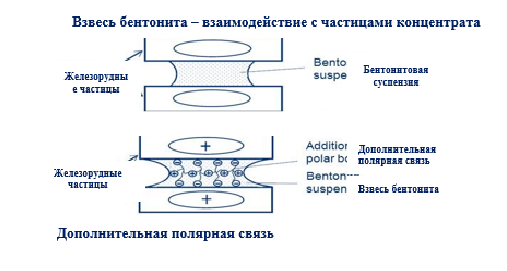
\includegraphics[width=\columnwidth]{media/chem2/image61}
	\caption*{Рис.1 - Взаимодействие бенто-полимерной суспензии с частицами концентрата}
\end{figure}

{\bfseries Материалы и методы.} Исследования по окомкованию
высококачественного железорудного концентрата АО «ССГПО» с применением
связующих добавок ТОО «Тагбент» на базе лаборатории ТОО «Алтайский
геолого-экологический институт» (ТОО «АГЭИ») были проведены лабораторные
испытания по окомкованию шихты с применением новых видов связующих.

\emph{Цель исследования:}

- проведение лабораторных исследований в лаборатории ТОО «АГЭИ» по
окомкованию с применением связующих добавок в составе шихты для
производства окатышей;

- выполнение тестов на окомкование и обжиг окатышей

- провести обжиг в лабораторных печах, способных смоделировать процесс
обжига

- оценка влияния связующих добавок на процесс сырого окомкования и их
физические свойства;

- определение оптимального расхода связующего при производстве окатышей;

- определение качественных характеристик сырых и обожженных окатышей,
полученных из железорудного концентрата АО «ССГПО» при использовании
выбранных бентонитовых глин и полимерных композиций, на основании
Методик, разработанных в ТОО «АГЭИ».

\emph{Основные задачи исследования:}

1. Разработать рецептуры шихтовки для получения обожженных окатышей с
улучшением физико-механических свойств.

2. Провести тестовые испытания для определения альтернативного связующего
для АО «ССГПО» при условии оптимального расхода бентонита.

3. Выявить влияния новых видов связующих на качество сырых, обожженных
окатышей.

4. Оценить свойства железорудных окатышей с новым составом шихты при
последующем металлургическом переделе.

5. Обосновать выбор оптимального связующего для проведения промышленных
испытаний.

В данной работе первый этап, который связан с определением показателей
качества шихты, проводился в лаборатории г. Усть-Каменогорск ТОО «АГЭИ»,
куда для проведения лабораторных испытаний была доставлена проба
железорудного концентрата АО «ССГПО» массой 100 кг.

Перед проведением испытаний по окомкованию шихты с новыми связующими
добавками были выполнены лабораторные исследования по определению
показателей качества компонентов шихты (железорудный концентрат,
бентонит, бенто-полимерная композиция).

Работы проводились с соблюдением требований ГОСТов, нормативной
документации, методических инструкций лаборатории ТОО «АГЭИ».

Отбор, подготовка проб шихтовых материалов для химического анализа
проводились согласно требованиям ГОСТ 15054. Результаты химического
анализа концентрата представлены в таблице 1.
\end{multicols}

\tcap{Таблица 1 - Показатели качества концентрата АО «ССГПО»}
\begin{longtblr}[
  label = none,
  entry = none,
]{
  cells = {c},
  cell{1}{1} = {r=2}{},
  cell{1}{2} = {r=2}{},
  cell{1}{3} = {c=2}{},
  vlines,
  hline{1,3-4} = {-}{},
  hline{2} = {3-4}{},
}
{Массовая \\доля влаги, \%} & {Массовая \\доля Feобщ., \%} & Массовая доля класса крупности (мм), \% & \\
 &  & -0,071 мм & -0,045\\
9,20 & 68,7 & 95,0 & 85,2
\end{longtblr}

Перед проведением лабораторных исследований выполнен полный химический
анализ шихтовых материалов (таблица 2).

\tcap{Таблица 2 - Химический состав шихтовых материалов}
\begin{longtblr}[
  label = none,
  entry = none,
]{
  width = \linewidth,
  colspec = {Q[256]Q[77]Q[69]Q[60]Q[58]Q[60]Q[71]Q[90]Q[183]},
  cells = {c},
  cell{1}{1} = {r=2}{},
  cell{1}{2} = {c=7}{},
  cell{1}{9} = {r=2}{},
  vlines,
  hline{1,3-6} = {-}{},
  hline{2} = {2-8}{},
}
Наименование материала & Массовая доля компонента, \% &  &  &  &  &  &  & Монтмор\-иллонит, \%\\
 & Fe\tsb{общ} & FeO & SiO\tsb{2} & CaO & MgO & Al\tsb{2}O\tsb{3} & п.п.п. & \\
Концентрат & 68,5 & 28,9 & 2,38 & 0,76 & 0,61 & 0,83 & 0,51 & -\\
Бентонит & 4,29 & 0,097 & 61,0 & 0,83 & 2,99 & 14,96 & 6,80 & 83,0\\
БПК & 3,70 & 1,65 & 60,8 & 1,37 & 2,33 & 18,3 & 8,4 & 75,5
\end{longtblr}

\begin{multicols}{2}
Показатели качества железорудного концентрата определяли по следующим
методикам:

массовая доля воды -- по ГОСТ 12764;

насыпная плотность -- по ГОС 25732 п.3;

истинная плотность -- по ГОСТ 26136 с использованием пикнометра АТС;

удельная поверхность концентрата - по ГОСТ 21043

Комкуемость определяли по методической инструкции лаборатории ТОО «АГЭИ»
разработанной на основе опытных исследований горнообогатительных
предприятий.

\emph{Определение комкуемости}

Методика заключается в определении скорости капиллярного распространения
воды в слое сухих тонкоизмельченных сыпучих материалов.

Комкуемость оказывает влияние на гранулометрический состав сырых
окатышей. Чем выше показатель комкуемости шихты, тем равномерней
формируется размер сырых окатышей, то есть выход годного класса в
диапазоне 10÷14 мм в общей массе полученных сырых окатышей
увеличивается.

Процесс получения сырого окатыша помимо динамических нагрузок в
окомкователе определяется, двумя основными типами силы -- молекулярной и
капиллярной. Эти же типы сил определяют закономерности пропитки слоя
концентрата. На рисунке 2 представлен фронт распространения воды в слое
концентрата.

\begin{figure}[H]
	\centering
	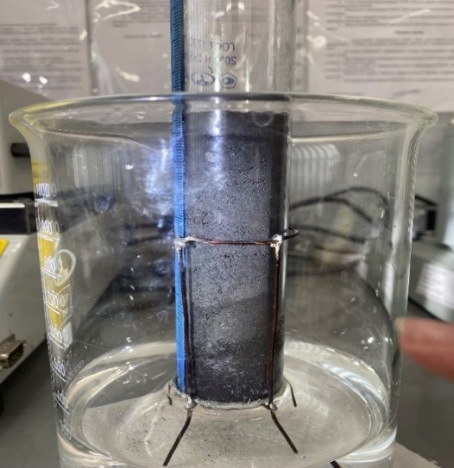
\includegraphics[width=0.9\columnwidth]{media/chem2/image62}
	\caption*{Рис.2 - Распределение воды в слое концентрата}
\end{figure}

Эффективный радиус (r ), в мкм рассчитывался по формуле (1):

\begin{equation}
r=\frac{4\cdot v\cdot l}{\sigma_H}\cdot \mu\cdot 1000,
\end{equation}

где: r -- радиус капиляра, мкм;

υ -- скорость капиллярного всасывания, см/сек;

l -- высота столбика жидкости в капилляре (11 см);

δ\textsubscript{н} -- коэффициент поверхности натяжения воды
(72,86⸱10\textsuperscript{-3}Н/м);

ƞ -- коэффициент вязкости воды (1,005).

\emph{Определение насыпной плотности}

Определение насыпной плотности концентрата проводилось в воздушно -
сухом состоянии без уплотнения согласно требованиям ГОСТ 25732 (п.3).
Согласно п.3.1.3 (таблица) для испытуемого материала крупность от 0 до 1
мм применялся цилиндрический сосуд вместимостью 5дм\textsuperscript{3}.

\emph{Определение истинной плотности}

Подготовка проб концентрата для определения истинной плотности
производились в соответствии с ГОСТ 26136 при использовании пикнометра
АТС.

Истинная плотность окатыша --- это плотность его твердой части, которая
определяется его химико-минералогическим составом, т.е. содержанием
железа общего.

\emph{Определение удельной поверхности концентрата}

Определение удельной поверхности концентрата проводилось на компьютерном
приборе ПСХ-12 М в соответствии с требованиями ГОСТ 21043.

Важным фактором, определяющим сцепление частиц и прочность сырых
окатышей, является величина удельной поверхности железорудного
концентрата.

Удельная поверхность напрямую связана с гранулометрическим составом
концентрата (чем больше доля мелких фракций, тем выше величина удельной
поверхности).

Удельная поверхность -- суммарная поверхность частиц в единице массы
материала без учета поверхности закрытых и открытых пор.

Физические свойства концентрата АО «ССГПО», поступившие в лабораторию
для исследований, были определены в лаборатории ТОО «АГЭИ». Значения
физических свойств концентрата представлены в таблице 3.
\end{multicols}

\tcap{Таблица 3 - Физические свойства концентрата АО «ССГПО»}
\begin{longtblr}[
  label = none,
  entry = none,
]{
  width = \linewidth,
  colspec = {Q[48]Q[106]Q[148]Q[146]Q[165]Q[113]Q[198]},
  rows = {font = \small},
  cells = {c},
  cell{1}{1} = {c=2}{},
  cell{1}{3} = {r=2}{},
  cell{1}{4} = {r=2}{},
  cell{1}{5} = {r=2}{},
  cell{1}{6} = {r=2}{},
  cell{1}{7} = {r=2}{},
  vlines,
  hline{1,3-4} = {-}{},
  hline{2} = {1-2}{},
}
Массовая доля, \% &  & Истинная	плотность, г/см\textsuperscript{3} & Насыпная плотность, т/м\textsuperscript{3} & Удельная поверхность, см\textsuperscript{2}/г & {
			Радиус
			капилляра,
			\\мкм
		} & {
			Скорость
			капиллярного всасывания,
			\\см/сек
		}\\
влага & кл.
			-0,040 мм &  &  &  &  & \\
8,94 & 82,6 & 4,905 & 2,0 & 1421 & 4,41 & 0,008
\end{longtblr}

\begin{multicols}{2}
Исследуемый концентрат АО «ССГПО» характеризуется высоким радиусом
капилляра (4,41мкм) и значительной скоростью капиллярного
распространения воды (0,008 см/сек) что указывает на хорошую комкуемость
данного концентрата и, как следствие, влияет на образование,
формирование и рост окатышей в процессе окомкования.

Показатели качества связующих добавок (бентонитовая глина и БПК)
определяли по следующим методикам:

- массовая доля песчаной фракции по ГОСТ 21216;

- глинистой составляющей по ГОСТ 28177;

- коллоидальность по ГОСТ 28177;

- массовая доля влаги по ГОСТ 28177;

- индекс набухания, по методическим инструкциям лаборатории ТОО «АГЭИ»;

- набухаемость, по методическим инструкциям лаборатории ТОО «АГЭИ»;

- эффективная вязкость 10\%\textsuperscript{} суспензии по
методическим инструкциям лаборатории ТОО «АГЭИ»;

Отбор проб и подготовка проводились согласно ГОСТ 28177, методическим
инструкциям, разработанных в институте.

Эффективная вязкость 10\% суспензии определялась на вискозиметре типа
FANN 35 SA, предварительно суспензия перемешивалась миксером Hamilton
Beach в течение 10 минут при скорости вращения мешалки
10~000мин\textsuperscript{-1}.

Результаты испытаний на показатели качества связующих, используемых при
получении экспериментальных партий железорудных окатышей представлены в
таблице 4.

Перед выполнением окомкования был проведен расчет шихтовых компонентов
для различных рецептур, представленный в таблице 5.
\end{multicols}

\tcap{Таблица 4 - Показатели качества связующих}
\begin{longtblr}[
  label = none,
  entry = none,
]{
  width = \linewidth,
  colspec = {Q[138]Q[46]Q[102]Q[133]Q[113]Q[144]Q[104]Q[144]},
  rows = {font = \small},
  cells = {c},
  cell{1}{1} = {r=2}{},
  cell{1}{2} = {c=3}{0.281\linewidth},
  cell{1}{5} = {r=2}{},
  cell{1}{6} = {r=2}{},
  cell{1}{7} = {r=2}{},
  cell{1}{8} = {r=2}{},
  vlines,
  hline{1,3-5} = {-}{},
  hline{2} = {2-4}{},
}
Наимен\-ование связующего & Массовая
				доля, \% &  &  & Коллои\-дальность,
				\% & Индекс
				набухания, мл/2г & Набухаем\-ость,
				раз & Эффективная
				вязкость, мПа⸱\\
 & влага & песчаная
				фракция & Глинистая
				составляющая &  &  &  & \\
бентонит & 21,91 & 1,5 & 98,0 & 75,0 & 52,4 & 15,3 & 90,0\\
БПК & 20,96 & 0,2 & 96,5 & 61,7 & 37,9 & 10,2 & 67,0
\end{longtblr}

\tcap{Таблица 5 - Расчет состава шихтовых компонентов}
\begin{longtblr}[
  label = none,
  entry = none,
]{
  width = \linewidth,
  colspec = {Q[277]Q[63]Q[63]Q[63]Q[63]Q[71]Q[63]Q[63]Q[63]Q[63]Q[63]},
  cells = {c},
  cell{1}{1} = {r=2}{},
  cell{1}{2} = {c=10}{0.637\linewidth},
  cell{2}{2} = {c=6}{0.386\linewidth},
  cell{2}{8} = {c=4}{0.252\linewidth},
  cell{3}{2} = {c=2}{0.126\linewidth},
  cell{3}{4} = {c=2}{0.126\linewidth},
  cell{3}{6} = {c=2}{0.134\linewidth},
  cell{3}{8} = {c=2}{0.126\linewidth},
  cell{3}{10} = {c=2}{0.126\linewidth},
  cell{4}{1} = {r=2}{},
  vlines,
  hline{1,3-4,6-8} = {-}{},
  hline{2,5} = {2-11}{},
}
Наименование показателей & Наименование связующего &  &  &  &  &  &  &  &  & \\
 & бентонит &  &  &  &  &  & БПК &  &  & \\
1 Расход связующего, \% & 0,30 &  & 0,40 &  & 0,50 &  & 0,30 &  & 0,40 & \\
2 Массовая доля влаги, \% & К & Б & К & Б & К & Б & К & БПК & К & БПК\\
 & 8,94 & 7,85 & 8,94 & 7,85 & 8,94 & 7,85 & 8,94 & 8,15 & 8,94 & 8,15\\
3 Дозировка на сухую массу, \% & 99,7 & 0,30 & 99,6 & 0,40 & 99,5 & 0,50 & 99,70 & 0,30 & 99,6 & 0,40\\
4 Дозировка на влажную массу, \% & 99,7 & 0,30 & 99,6 & 0,40 & 99,49 & 0,510 & 99,7 & 0,30 & 99,6 & 0,30
\end{longtblr}
\vspace{-2em}
\tcap{\normalfont\emph{Примечание: К -- концентрат, Б - бентонит}}

Испытания по окомкованию шихты проводились согласно требованиям
методической инструкции лаборатории ТОО «АГЭИ». На рисунке 3 приведена
схема проведения испытаний.

\begin{figure}[H]
	\centering
	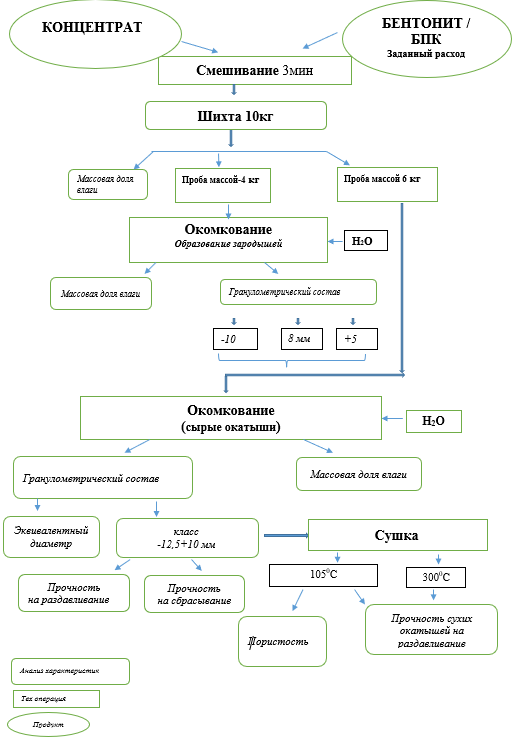
\includegraphics[width=0.6\textwidth]{media/chem2/image64}
	\caption*{Рис.3 - Схема проведения процесса окомкования}
\end{figure}
\vspace{-2em}
\begin{multicols}{2}
Полученные окатыши выгружались из окомкователя для проведения
физико-механических испытаний.

В образцах сырых окатышей определяли следующие показатели:

- массовая доля влаги согласно ГОСТ 12764;

- гранулометрический состав согласно ГОСТ 27562

- прочность на раздавливание сырых и высушенных в сушильном шкафу
окатышей при температуре сушки 105\textsuperscript{о}С и
300\textsuperscript{о}С на ИПГ-1;

- прочность на сбрасывание с высоты 500 мм на резиновую и металлическую
поверхности;

- пористость высушенных окатышей по ГОСТ 25732.

После термообработки обожженные окатыши подвергали испытаниям на
определение следующих показателей:

- прочность на сжатие на испытательной машине ИТС-8313-1,0 по ИСО 4700;

- прочность на удар и истираемость в мини-барабане по ГОСТ 15137;

- пористость по ГОСТ 25732 на весах VIBRA AJH 420 CE с комплектом
измерителя плотности AJDK.;

- определение химического состава (Feобщ, FeO, SiO2, CaO, MgO,
Al\textsubscript{2}O\textsubscript{3}, потери при прокаливании).

На рисунке 4 представлена лабораторная установка позволяющая проводить
спекание исследуемых окатышей в изокинетических условиях. Термообработка
тестовых проб на такой установке приближена к условиям действующих
обжиговых машин конвейерного типа.

{\bfseries Результаты и обсуждение.} Результаты лабораторных испытаний
окатышей, полученных при окомковании высококачественного концентрата с
добавлением различных связующих с разным процентом вложения представлены
в таблице 6, рисунках 5 - 6.
\end{multicols}

\begin{figure}[H]
	\centering
	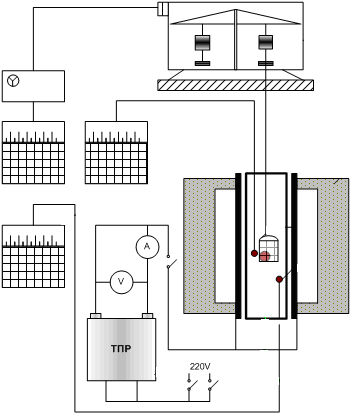
\includegraphics[width=0.6\textwidth,height=0.5\textwidth]{media/chem2/image65}
	\caption*{Рис.4 -Схема лабораторной установки спекания окатышей в изокинетических условиях}
\end{figure}

\tcap{Таблица 6 - Результаты лабораторных испытаний окатышей из концентрата АО «ССГПО» полученных с применением разными связующих}
\begin{longtblr}[
  label = none,
  entry = none,
]{
  width = \linewidth,
  colspec = {Q[465]Q[106]Q[106]Q[106]Q[73]Q[73]},
  row{1} = {c},
  row{2} = {c},
  column{3} = {c},
  column{4} = {c},
  column{6} = {c},
  cell{1}{1} = {r=2}{},
  cell{1}{2} = {c=5}{0.464\linewidth},
  cell{2}{2} = {c=3}{0.318\linewidth},
  cell{2}{5} = {c=2}{0.146\linewidth},
  cell{3}{2} = {c},
  cell{3}{5} = {c},
  cell{4}{2} = {c},
  cell{4}{5} = {c},
  cell{5}{2} = {c},
  cell{5}{5} = {c},
  cell{6}{2} = {c},
  cell{6}{5} = {c},
  cell{7}{2} = {c},
  cell{7}{5} = {c},
  vlines,
  hline{1,3-8} = {-}{},
  hline{2} = {2-6}{},
}
Наименование
				показателей & Наименование
				связующего &  &  &  & \\
 & ТОО
				«ТАГБЕНТ» (бентонит) &  &  & БПК & \\
Расход
				связующего, \% & 0,30 & 0,40 & 0,50 & 0,30 & 0,40\\
{
				Массовая
				доля влаги, \%
				\\-
				сырые окатыши
			} & 8,20 & 8,31 & 8,27 & 8,14 & 8,19\\
{
				Массовая
				доля класса крупности (мм), \%
				\\
				+16
				\\
				-16
				+14
				\\
				-14
				+12,5
				\\
				-12,5
				+11,2
				\\
				-11,2
				+10
				\\
				-10
				+8
				\\
				-
				8 +5
				\\-
				5 +0
			} & {
				0,2
				\\
				1,2
				\\
				8,2
				\\
				34,2
				\\
				25,0
				\\
				27,2
				\\
				4,0
				\\0,0
			} & {
				0,8
				\\
				2,6
				\\
				21,2
				\\
				43,4
				\\
				20,3
				\\
				10,4
				\\
				1,3
				\\0,0
			} & {
				0,4
				\\
				5,3
				\\
				28,4
				\\
				45,1
				\\
				14,0
				\\
				6,0
				\\
				0,8
				\\0,0
			} & {
				0,0
				\\
				1,4
				\\
				6,7
				\\
				34,2
				\\
				30,5
				\\
				23,5
				\\
				3,7
				\\0,0
			} & {
				0,0
				\\
				3,4
				\\
				18,4
				\\
				41,9
				\\
				22,1
				\\
				12,1
				\\
				2,1
				\\0,0
			}\\
Диаметр
				сырых окатышей, мм & 10,34 & 11,28 & 11,68 & 10,40 & 11,15\\
Пористость
				сухих окатышей, \% & 32,1 & 31,7 & 30,8 & 31,5 & 30,2
\end{longtblr}

\begin{multicols}{2}
Анализ полученных данных свидетельствует о том, что наибольший выход
годного класса окатышей (класс крупности -12,5 мм + 10 мм) при расходе
0,3-0,4\% дают БПК. При этом массовая доля влаги сырых окатышей
сохраняется на уровне 8 \%.

Следует отметить, что выход годного класса при введении 0,3\% связующего
в случае БПК на 4,2 \% выше, чем при использовании чистого бентопорошка.
\end{multicols}

\begin{figure}[H]
	\centering
	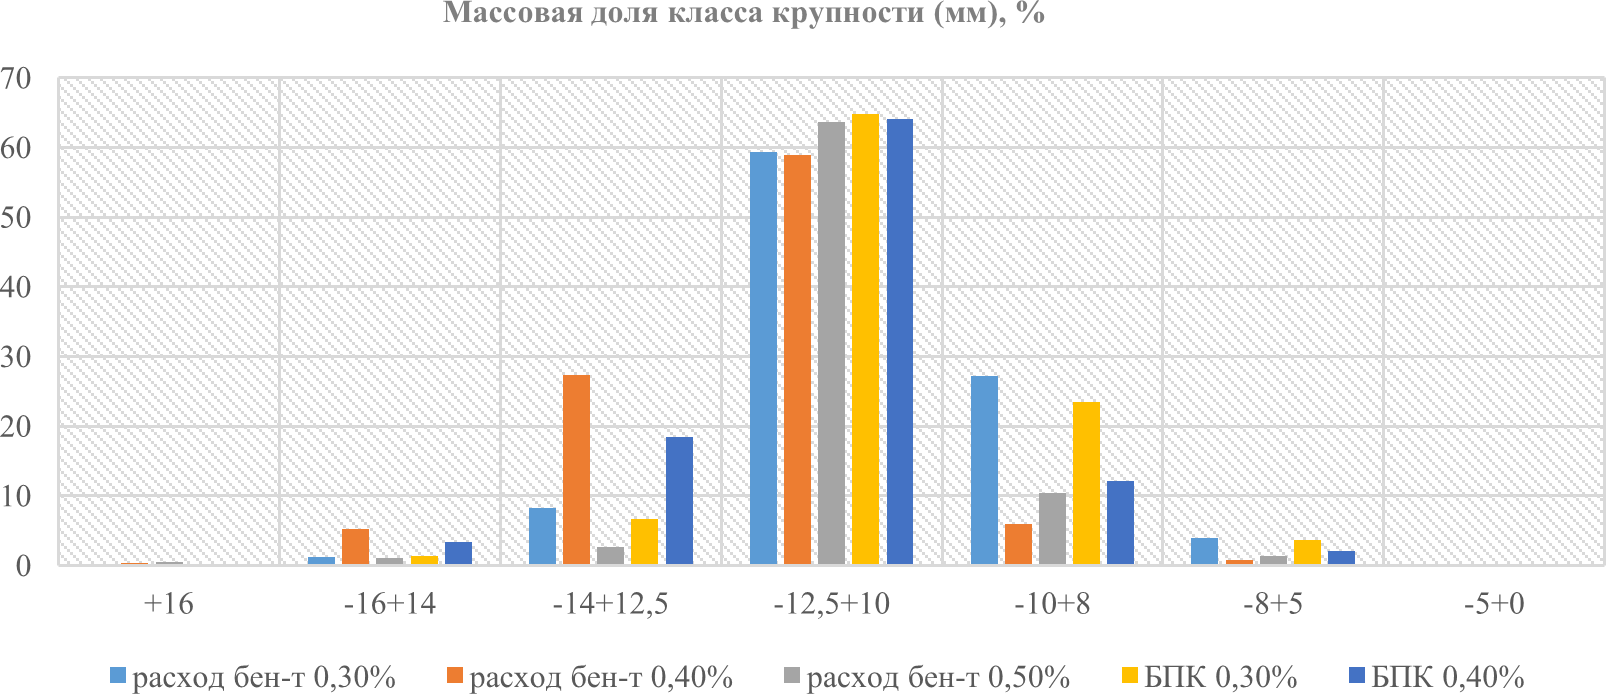
\includegraphics[width=0.8\textwidth]{media/chem4/image7}
	\caption*{Рис.5 - Гранулометрический состав сырых окатышей}
\end{figure}

\begin{multicols}{2}
Результаты испытаний сухих окатышей на пористость свидетельствуют о
преобладании открытых пор при их равномерном распределении в объёмах.

Процесс окомкования при применении БПК в лабораторных условиях проходит
стабильно. Содержание воды в компонентах шихты и добавляемой достаточное
для получения необходимой вязкости и протекания процесса окомкования
(для формирования равномерной и прочной структуры окатыша).

Поскольку расход бентонита/БПК (0,5/0,4 \%) удовлетворяет техническим
требованиям по прочностным свойствам сырых окатышей (рисунок 6),
дальнейшее увеличение расхода связующего было нецелесообразно.

Термообработка тестовых проб была приближена к условиям действующей
обжиговой машины конвейерного типа при производстве Dr-окатышей.
Максимальная достигаемая температура в печи составила 1300
\textsuperscript{о}С.

Данные физико-химических свойств обожженных окатышей, полученных после
обжига приведены в таблице 7.
\end{multicols}

\begin{figure}[H]
	\centering
	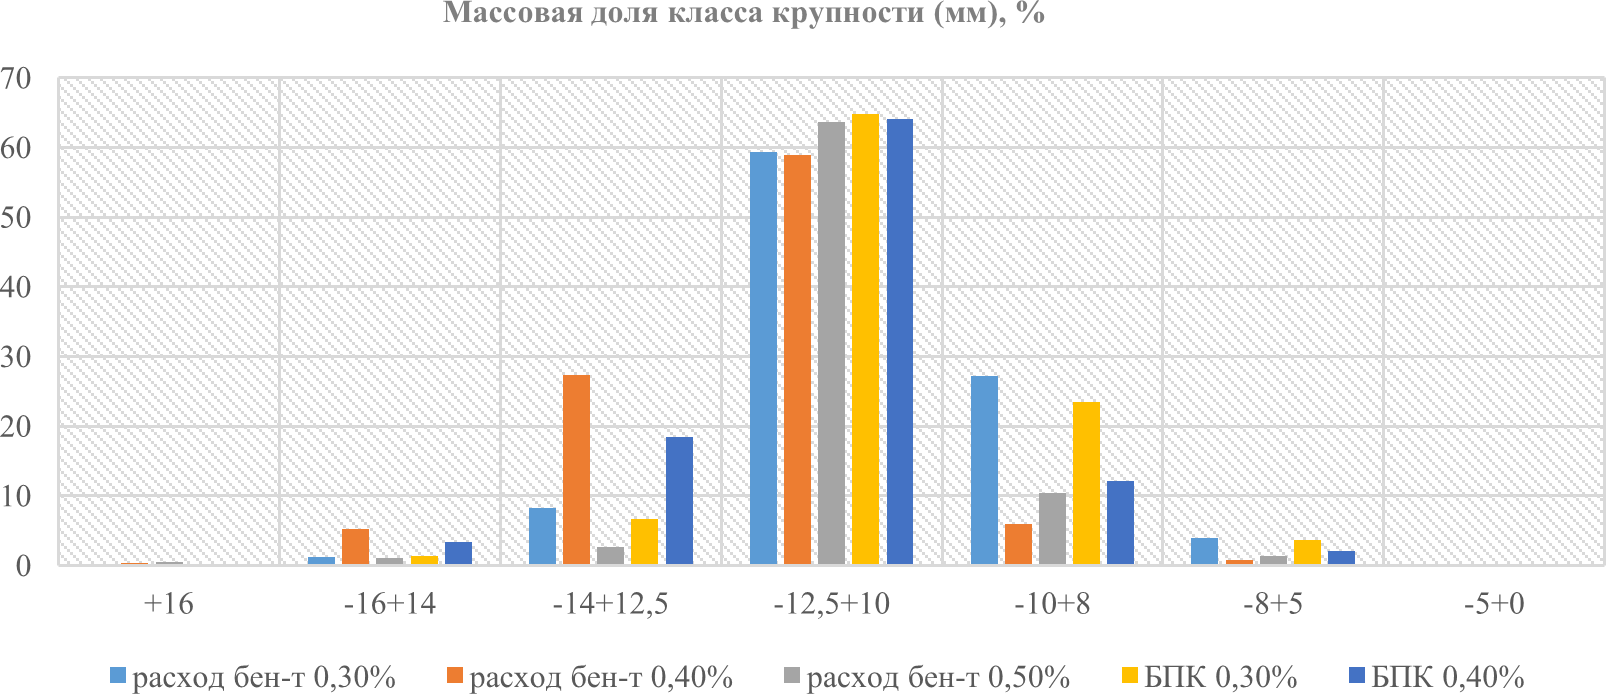
\includegraphics[width=0.8\textwidth]{media/chem4/image7}
	\caption*{Рис.6 - Прочностные характеристики сырых и сухих окатышей}
\end{figure}

\tcap{Таблица 7 - Физико-химические свойства обожженных окатышей}
\begin{longtblr}[
  label = none,
  entry = none,
]{
  width = \linewidth,
  colspec = {Q[113]Q[88]Q[60]Q[88]Q[67]Q[60]Q[65]Q[50]Q[50]Q[50]Q[52]Q[60]Q[62]Q[48]},
  rows = {font = \scriptsize},
  cells = {c},
  cell{1}{1} = {r=2}{},
  cell{1}{2} = {r=2}{},
  cell{1}{3} = {c=3}{0.215\linewidth},
  cell{1}{6} = {r=2}{},
  cell{1}{7} = {c=8}{0.437\linewidth},
  cell{3}{1} = {r=3}{},
  cell{6}{1} = {r=2}{},
  vlines,
  hline{1,3,6,8} = {-}{},
  hline{2} = {3-5,7-14}{},
  hline{4-5,7} = {2-14}{},
}
Наименова\-ние связующего & Расход, связующей добавки, \% & Прочностные характеристики обожжённых окатышей &  &  & Порист\-ость, \% & Химический состав, \% &  &  &  &  &  &  & \\
 &  & на				удар (Б\textsuperscript{+5}),				\% & сопротив\-ление истиранию (Б\textsuperscript{-0,5}), \% & на сжатие, кг/ок. &  & Fe\tsb{общ} & FeO & SiO\tsb{2} & CaO & MgO & Al\tsb{2}O\tsb{3} & S & nnn\\
Бентонит & 0,30 & 97,5 & 2,5 & 306,0 & 22,6 & 66,55 & 0,72 & 2,61 & 0,55 & 0,71 & 0,96 & 0,0022 & 0,23\\
 & 0,40 & 98,0 & 2,0 & 314,0 & 21,7 & 66,44 & 0,66 & 2,70 & 0,51 & 0,71 & 0,99 & 0,0018 & 0,19\\
 & 0,50 & 98,2 & 1,8 & 392,0 & 21,2 & 66,34 & 0,82 & 2,72 & 0,55 & 0,71 & 1,00 & 0,0017 & 0,22\\
БПК & 0,30 & 97,6 & 2,4 & 279,0 & 23,3 & 66,60 & 0,82 & 2,61 & 0,49 & 0,70 & 0,99 & 0,0021 & 0,23\\
 & 0,40 & 98,1 & 1,9 & 318,0 & 22,8 & 66,34 & 0,94 & 2,68 & 0,52 & 0,70 & 0,99 & 0,0022 & 0,20
\end{longtblr}

\begin{multicols}{2}
При обжиге одновременно происходят процессы образования пор в результате
выделения газов при разложении гидратов и карбонатов, также происходит
разрушение первоначальных пустот или их перераспределение вокруг
контактов зерен окатышей. Часть пор заплавляется, другая часть
укрупняется за счет мелких, появляются поры на поверхности окатышей.

Контролируя температуру обжига, а также учитывая плавкость шихтовых
компонентов и количество выделяемых газов можно получить структуру с
большей или меньшей пористостью.

Наибольшее влияние температура обжига оказывает на пористость окатышей в
период твердофазного спекания и во время перехода к жидкофазному
спеканию. При отсутствии жидкой фазы при твердофазном спекании
увеличивается число контактов рудных зерен и, как следствие, пористость
уменьшается.

В свою очередь пористость напрямую способствует:

- улучшению способности к восстановлению;

- упрощению сброса газа при обжиге;

- сохранению механических свойств.

Анализ результатов исследования прочностных характеристик обожженных
окатышей свидетельствует о том, что оптимальный расход связующего, при
условии постоянства остальных компонентов шихты, находится в пределах
0,3-0,4 \%, при этом при расходе 0,4 \% холодная прочность обожженных
окатышей с применением БПК на 2,2 \% выше, чем при использовании
бентонитовой глины.

При оценке прочностных свойств сухих и обожженных окатышей была выявлена
линейная зависимость между расходом связующего и характеристиками
окатышей. С ростом оптимального удельного расхода связующего
увеличивается прочность обожженных окатышей с одновременным обеспечением
заданных показателей качества окатышей. В целом, по результатам
исследований, можно отметить, что физико-механические свойства
обожженных окатышей зависят от качества сырых окатышей, на которые кроме
комплекса других факторов, влияют свойства связующего.

Рекомендуемые связующие добавки в виде бентопорошка ТОО «Тагбент» и БПК
при расходе в шихту 0,4 \% позволяют стабилизировать гранулометрический
состав сырых окатышей, улучшить прочностные характеристики сырых, сухих
и обожженных окатышей, улучшить показатель сопротивления истиранию
обожженных окатышей.
\end{multicols}

\begin{figure}[H]
	\centering
	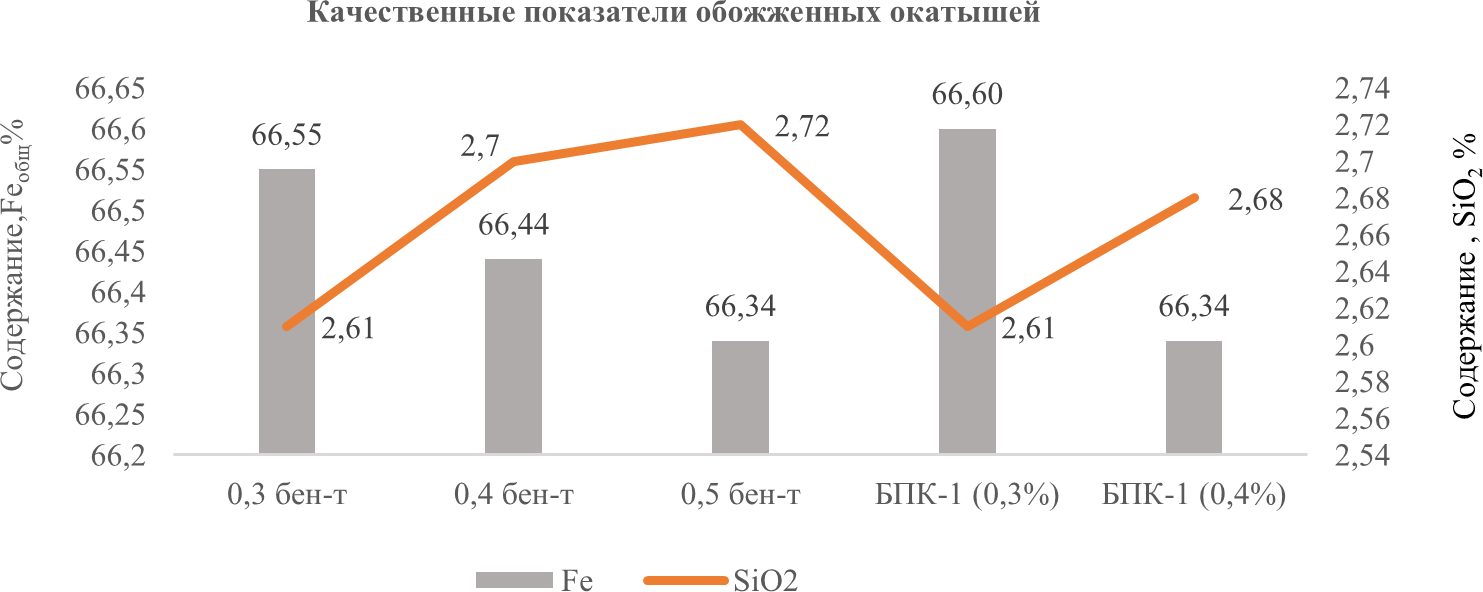
\includegraphics[width=0.8\textwidth]{media/chem4/image9}
	\caption*{Рис.7 - Качественные характеристики обожженных окатышей}
\end{figure}

\begin{multicols}{2}
Анализ полученных обожженных окатышей показывает, что при оптимально
выбранном удельном расходе бентонита увеличивается не только прочность
обожженных окатышей, но также снижается содержание вредных примесей
SiO\textsubscript{2}, а содержание ценного компонента --Fe
увеличивается.

{\bfseries Выводы.} Выполненные исследования позволили определить роль
предложенных связующих веществ: бентонита и бенто-полимерной композиции
ТОО «Тагбент» в составе шихты, соответствующего типа и дозировки при
производстве железорудных окатышей из высококачественного концентрата АО
«ССГПО».

В ходе тестовых лабораторных испытаний был установлен состав и дозировка
связующих компонентов в составе шихты.

Установлена прямая зависимость прочности обожжённых окатышей от
прочности сухих, однако, при проведении опытно-промышленных испытаний в
условиях производства необходимо учитывать, что в ходе движения слоя на
обжиговой машине возникают большие слоевые нагрузки и деформация
окатышей, получивших внутренние «незалеченные» дефекты в процессе
транспортировки и укладки выше, чем в лабораторных условиях.

Показано, что для получения необходимой вязкости (для склеивания
окатыша) гелеобразной смеси (коллоида) бентонита и воды (для
формирования равномерной и прочной структуры сырого окатыша) необходимо
достаточное количество воды в шихте, подаваемой на сырое окомкование.
Это способствует стабильности процесса окомкования, удерживанию большей
части влаги, создавая тем самым гладкую поверхность окатыша.

Установлено, что применение высококачественных связующих позволяет
получать железорудные окатыши с высокой прочностью на сжатие и низким
сопротивлением к истиранию (Б\textsuperscript{-0,5}), с заданными
качественными показателями окатышей.
\end{multicols}

\begin{center}
{\bfseries Литература}
\end{center}

\begin{references}
1. Автоматизация металлургического производства / электронный учебник --
Карагандинский государственный технический университет URL:
\href{https://www.kstu.kz/wp-content/uploads/2018/05/tsifrovaya-mitallurgiya/el-uch-po-ampr/index.htm-}{https://www.kstu.kz}
Дата обращения: 13.02.2025.

2. Тимофеева А.С., Никитченко Т.В., Федина В.В. Определение комкуемости
железорудной шихты с целью прогнозирования прочностных свойств окатышей
// Современные наукоемкие технологии. -2015.-№ 8.- С.53-57

3. Фирсовская Е.В., Паринова А.С., Тимофеева А.С. Комкуемость шихты и
прочность окатышей в зависимости от удельной поверхности концентрата
//Материалы IX Международной студенческой научной конференции
«Студенческий научный форум» URL:
\href{https://scienceforum.ru/2017/article/2017038139}{https://scienceforum.ru} .-Дата обращения:
14.02.2025.

4. Жунусов А.К., Кулумбаев Н.К., Нурмаганбетов Ж.О., Толымбекова Л.Б.
Производство хроморудных окатышей из мелкодисперсных отходов // Наука и
техника Казахстана. - 2007. - № 3. - С.39-44.

5. Юрьев Б.П., Спирин Н.А., Шешуков О.Ю., Гольцев В.А., Шевченко О.И.,
Метелкин А.А. Разработка технологий для производства железорудных
окатышей с высокими металлургическими свойствами: научная
монография.-Нижний Тагил:НТИ(филиал) УрФУ, 2018 - 172 с. ISBN
978-5-9544-0091-5

6. Шаврин А.В. Исследование и разработка технологических решений по
улучшению металлургических свойств окатышей на основе оптимизации их
структуры {[}Текст{]} : автореф. дис. ... канд. техн. наук: 05.16.02 /.
- Екатеринбург : {[}б. и.{]}, 2006. - 24 с.

7. Байджанов Д.О., Дивак Л.А., Рожков А.В., Ахметов Б.Б. Вяжущие
вещества: учебное пособие / Карагандинский государственный технический
университет. - Караганда: Изд-во Санат, 2019. - 90 с. ISBN(onlain)
978-9965-38-402-8

8. Ibraimova D. M-K., Rozhkova O.V., Musabekov K.B., Tazhibayeva S.M.,
Rozhkov V., Yermekov M.T. Development of Methods to Obtain Composite
Materials from Organoclays //Eurasian Journal of Chemistry. -2023.
-Vol.28 № 4(112).- P.101-111. DOI 10.31489/2959-0663/4-23-14

9. Рожкова О.В., Муздыбаева Ш.А., Мусабеков К.Б., Ибраимова Д. М., Рожков
В.И., Ермеков М.Т. Разработка методов получения носителей лекарственных
средств на основе органомодифицированных глин // Известия Национальной
академии наук Республики Казахстан. Серия химических наук. -2023 -№ 3.
-- C.138-156. DOI 10.32014/2023.2518-1491.183

10. Musabekov K.B., Rozhkova O.V., Artykova (Ibraimova) D. M-K., Yermekov
M.T., Muzdybaeva Sh.A. Application of bentonite clay as a protective
barrier in the disposal of radioactive waste of nuclear industry of
Kazakhstan // Известия Национальной академии наук Республики Казахстан.
Серия Химия и технология. -2023. - Vol.1(454).- P.66-77.
\href{https://doi.org/10.32014/2023.2518-1491.148}{DOI 10.32014/2023.2518-1491.148}
\end{references}

\begin{center}
{\bfseries References}
\end{center}

\begin{references}
1. Avtomatizatsiya metallurgicheskogo proizvodstva / elektronnyi uchebnik
-- Karagandinskii gosudarstv\-ennyi tekhnicheskii universitet URL:
\href{https://www.kstu.kz/wp-content/uploads/2018/05/tsifrovaya-mitallurgiya/el-uch-po-ampr/index.htm-}{https://www.kstu.kz}
Data obrashcheniya: 13.02.2025. {[}in Russian{]}

2. Timofeeva A.S., Nikitchenko T.V., Fedina V.V. Opredelenie komkuemosti
zhelezorudnoj shihty s cel' ju prognozirovanija
prochnostnyh svojstv okatyshej // Sovremennye naukoemkie tehnologii.
-2015.-№ 8.- S.53-57. {[}in Russian{]}

3. Firsovskaja E.V., Parinova A.S., Timofeeva A.S.
Komkuemost'{} shihty i prochnost'{}
okatyshej v zavis\-imosti ot udel' noj poverhnosti
koncentrata //Materialy IX Mezhdunarodnoj studencheskoj nauchnoj
konf\-erencii «Studencheskij nauchnyj forum» URL:
\href{https://scienceforum.ru/2017/article/2017038139}{https://scienceforum.ru} .-Data obrashhenija:
14.02.2025. {[}in Russian{]}

4. Zhunusov A.K., Kulumbaev N.K., Nurmaganbetov Zh.O., Tolymbekova L.B.
Proizvodstvo hromorudnyh okatyshej iz melkodispersnyh othodov // Nauka i
tehnika Kazahstana. - 2007. - № 3. - S.39-44. {[}in Russian{]}

5. Jur' ev B.P., Spirin N.A., Sheshukov O.Ju.,
Gol' cev V.A., Shevchenko O.I., Metelkin A.A. Razrabotka
tehnologij dlja proizvodstva zhelezorudnyh okatyshej s vysokimi
metallurgicheskimi svojstvami: nauchnaja monografija.-Nizhnij
Tagil:NTI(filial) UrFU, 2018 - 172 s. ISBN 978-5-9544-0091-5. {[}in
Russian{]}

6. Shavrin A.V. Issledovanie i razrabotka tehnologicheskih reshenij po
uluchsheniju metallurgicheskih svojstv okatyshej na osnove optimizacii
ih struktury {[}Tekst{]} : avtoref. dis. ... kand. tehn. nauk: 05.16.02
/. - Ekaterinburg : {[}b. i.{]}, 2006. - 24 s. {[}in Russian{]}

7. Bajdzhanov D.O., Divak L.A., Rozhkov A.V., Ahmetov B.B. Vjazhushhie
veshhestva: uchebnoe posobie / Karagandinskij gosudarstvennyj
tehnicheskij universitet. - Karaganda: Izd-vo Sanat, 2019. - 90 s.\\
ISBN(onlain) 978-9965-38-402-8. {[}in Russian{]}

8. Ibraimova D. M-K., Rozhkova O.V., Musabekov K.B., Tazhibayeva S.M.,
Rozhkov V., Yermekov M.T. Development of Methods to Obtain Composite
Materials from Organoclays //Eurasian Journal of Chemistry. -2023.
-Vol.28 № 4(112).- P.101-111. DOI 10.31489/2959-0663/4-23-14

9. Rozhkova O.V., Muzdybaeva Sh.A., Musabekov K.B., Ibraimova D. M.,
Rozhkov V.I., Ermekov M.T. Razrabotka metodov poluchenija nositelej
lekarstvennyh sredstv na osnove organomodificirovannyh glin // Izvestija
Nacional' noj akademii nauk Respubliki Kazahstan. Serija
himicheskih nauk. -2023 -№ 3. -- C.138-156. DOI
10.32014/2023.2518-1491.183. {[}in Russian{]}

10. Musabekov K.B., Rozhkova O.V., Artykova (Ibraimova) D. M-K., Yermekov
M.T., Muzdybaeva Sh.A. Application of bentonite clay as a protective
barrier in the disposal of radioactive waste of nuclear industry of
Kazakhstan // Известия Национальной академии наук Республики Казахстан.
Серия Химия и технология. -2023. - Vol.1(454).- P.66-77.
\href{https://doi.org/10.32014/2023.2518-1491.148}{DOI 10.32014/2023.2518-1491.148}
\end{references}

\begin{authorinfo}
\hspace{1em}\emph{{\bfseries Сведения об авторах}}  

Рожкова О.В. — доктор химических наук, профессор, академик
Национальной академии естественных наук Республики Казахстан, НАО
«Казахский агротехнический исследовательский университет
им. С. Сейфуллина», Астана, Казахстан, АО «Science and Technology
Solutions», Астана, Казахстан, e-mail: rozhkova.o@stsolutions.kz;

Ковалёва О.О. — магистр по ядерной энергетике и теплофизике, директор
ТОО "Алтайский геолого-экологический институт", Усть-Каменогорск,
Казахстан, e-mail: kovaleva@agikaz.pro;

Лебедева В.И. — заместитель генерального директора по стратегическому
развитию ООО «Бентонит Хакасии», Россия, г. Черногорск, Республика
Хакасия, e-mail: lebedeva@bentonit.ru;

Ветюгов Д.А. — менеджер по развитию ООО «Компания Бентонит»,
г. Москва, Россия, e-mail: da.vetugov@bentonit.ru;

Рожков В.И. — кандидат технических наук, НАО «Казахский
агротехнический университет им. С. Сейфуллина», г. Астана, Казахстан,
e-mail: vitalrza1983@gmail.com.

\hspace{1em}\emph{{\bfseries Information about the authors}}  

O.V. Rozhkova — Doctor of Chemical Sciences, Professor, Academician of
the National Academy of Natural Sciences of the Republic of
Kazakhstan, NAO "Kazakh Agrotechnical Research University named after
S. Seifullin", Astana, Kazakhstan, JSC "Science and Technology
Solutions", Astana, Kazakhstan, e-mail: rozhkova.o@stsolutions.kz;

O.O. Kovaleva — Master of Nuclear Energy and Thermophysics, Director
of LLP "Altai Geological-Ecological Institute", Ust-Kamenogorsk,
Kazakhstan, e-mail: kovaleva@agikaz.pro;

V.I. Lebedeva — Deputy General Director for Strategic Development, LLC
"Bentonite Khakassia", Russia, Chernogorsk, Republic of Khakassia,
e-mail: lebedeva@bentonit.ru;

D.A. Vetyugov — Development Manager, LLC "Bentonite Company", Moscow,
Russia, e-mail: da.vetugov@bentonit.ru;

V.I. Rozhkov — Candidate of Technical Sciences, NAO "Kazakh
Agrotechnical University named after S. Seifullin", Astana,
Kazakhstan, e-mail: vitalrza1983@gmail.com.
\end{authorinfo}
